\documentclass[oneside]{report}
\usepackage[parfill]{parskip}

\usepackage{hyperref}

\usepackage{enumitem}

\usepackage{listings}
\lstset{tabsize=3, numbers=left, basicstyle=\ttfamily, escapeinside=~~, xleftmargin=-1cm}
\let\origthelstnumber\thelstnumber
\makeatletter
\newcommand*\Suppressnumber{%
	\lst@AddToHook{OnNewLine}{%
		\let\thelstnumber\relax%
		\advance\c@lstnumber-\@ne\relax%
	}%
}
\makeatother

\usepackage{tikz}
\usetikzlibrary{arrows.meta}
\usetikzlibrary{er}  % entity-relationship diagram
\usetikzlibrary{positioning}

\renewcommand{\familydefault}{\sfdefault}
\Suppressnumber
\begin{document}
\begin{center}
\textbf{COMP3700 Activity 5}\\
Tripp Isbell\\
cai0004@auburn.edu
\end{center}
\begin{enumerate}[itemindent=-2cm]
	\item Draw entity-relationship diagram
	
	\hskip-3cm\resizebox{18cm}{4cm}{%
		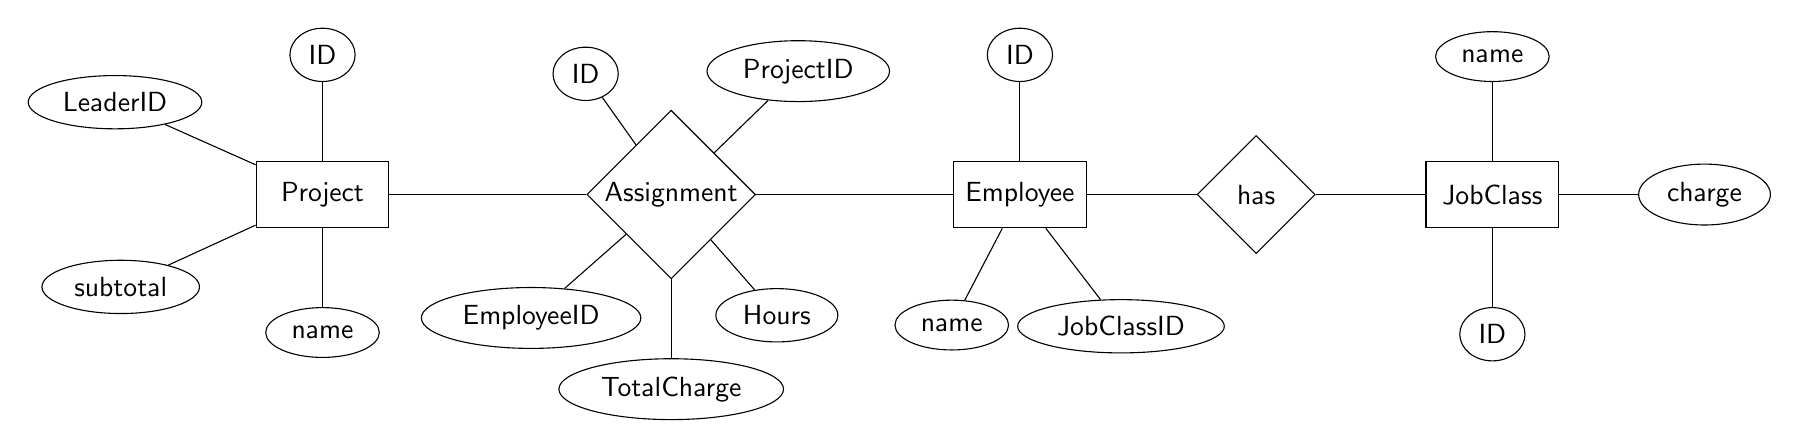
\begin{tikzpicture}[node distance=3cm]
			\node[entity] (Project)					{Project};
			\node[relationship] (Assignment) [right=2.5cm of Project] {Assignment}
				edge (Project);
			\node[entity] (Employee) [right=2.5 of Assignment]	{Employee}
				edge (Assignment);
			\node[relationship] (has) [right of=Employee, minimum size=1.5cm]		{has}
				edge (Employee);
			\node[entity] (JobClass) [right of=has]			{JobClass}
				edge (has);
				
			\node[attribute] (ProjectID) [above=1cm of Project] {ID} edge (Project);
			\node[attribute] (ProjectName) [below=1cm of Project] {name} edge (Project);
			\node[attribute] (subtotal) [below left=0.5cm and 1cm of Project] {subtotal} edge (Project);
			\node[attribute] (ProjectLeaderID) [above left=0.5cm and 1cm of Project] {LeaderID} edge (Project);
			
			\node[attribute] (EmployeeID) [above=1cm of Employee] {ID} edge (Employee);
			\node[attribute] (EmployeeName) [below left=1cm and -0.5cm of Employee] {name} edge (Employee);
			\node[attribute] (EmployeeJobClassID) [below right=1cm and -0.5cm of Employee] {JobClassID} edge (Employee);
			
			\node[attribute] (JobClassID) [below=1cm of JobClass] {ID} edge (JobClass);
			\node[attribute] (JobClassName) [above=1cm of JobClass] {name} edge (JobClass);
			\node[attribute] (JobClassCharge) [right=1cm of JobClass] {charge} edge (JobClass);
			
			\node[attribute] (AssignmentID) [above left=0.75cm and 0.25cm of Assignment] {ID} edge (Assignment);
			\node[attribute] (AssignmentProjectID) [above right=0.75cm and 0.25cm of Assignment] {ProjectID} edge (Assignment);
			\node[attribute] (AssignmentEmployeeID) [below left=0.75cm and 0.25cm of Assignment] {EmployeeID} edge (Assignment);
			\node[attribute] (AssignmentHoursBilled) [below right=0.75cm and 0.25cm of Assignment] {Hours} edge (Assignment);
			\node[attribute] (AssignmentTotalCharge) [below=1cm of Assignment] {TotalCharge} edge (Assignment);
			
		\end{tikzpicture}
	}
	
	\item Convert to schema (relations with attributes and keys)
	
	\begin{itemize}[itemindent=-1.5cm]
		\item Project (ProductID, name, subtotal, ProjectLeaderID)
		\item Employee (EmployeeID, name, JobClassID)
		\item JobClass (JobID, name, chargePerHour)
		\item Assignment (AssignID, ProjectID, EmployeeID, HoursBilled, TotalCharge)
	\end{itemize}
	\item Write SQL code to define those tables
	
\begin{lstlisting} 
CREATE TABLE Project (
	ProjectID int NON NULL PRIMARY KEY,
	Name varchar(100),
	Subtotal float,
	ProjectLeaderID int FOREIGN KEY REFERENCES Employee(EmployeeID)
);

CREATE TABLE Employee (
	EmployeeID int NON NULL PRIMARY KEY,
	Name varchar(100),
	JobClassID int FOREIGN KEY REFERENCES JobClass(JobClassID)
);

CREATE TABLE JobClass (
	JobClassID int NON NULL PRIMARY KEY,
	Name varchar(100),
	Charge float,
);
~\newpage~
CREATE TABLE Assignment (
	AssignID int NON NULL primary key,
	ProjectID int FOREIGN KEY REFERENCES Project(ProjectID),
	EmployeeID int FOREIGN KEY REFERENCES Employee(EmployeeID),
	Hours int,
	TotalCharge float
);
\end{lstlisting}
	
	\item Write SQL to insert the data into those tables
	
\begin{lstlisting}

INSERT INTO Project (ProjectID, Name, Subtotal, ProjectLeaderID)
VALUES(15, 'Evergreen', 10549.70, 105),
		(18, 'Amber Wave', 7171.47, 104),
		(22, 'Rolling Tide', 13660.10, 113),
		(25, 'Starflight', 17559.82, 101);
		
INSERT INTO JobClass (JobClassID, Name, Charge)
VALUES(1, 'Elec. Engineer', 84.50),
		(2, 'Database Designer', 105.00),
		(3, 'Programmer', 35.75),
		(4, 'Systems Analyst', 96.75),
		(5, 'Applications Designer', 48.10),
		(6, 'General Support', 18.36),
		(7, 'DSS Analyst', 45.95),
		(8, Clerical Support', 26.87);
		
INSERT INTO Employee (EmployeeID, Name, JobClassID)
VALUES(101, 'John G. News', 2),
		(102, 'David H. Senior, 4),
		(103, 'June E. Arbough', 1),
		~$\vdots$~

INSERT INTO Assignment (AssignID, ProjectID, EmployeeID, Hours, TotalCharge)
VALUES(1, 15, 103, 23.8, 2011.10),
		(2, 15, 101, 19.4, 2037.00),
		~$\vdots$~
\end{lstlisting}

\end{enumerate}
\end{document}